\documentclass[12pt,a4paper]{article}

\usepackage[a4paper,text={16.5cm,25.2cm},centering]{geometry}
\usepackage{lmodern}
\usepackage{amssymb,amsmath}
\usepackage{bm}
\usepackage{graphicx}
\usepackage{microtype}
\usepackage{hyperref}
\setlength{\parindent}{0pt}
\setlength{\parskip}{1.2ex}

\hypersetup
       {   pdfauthor = { Sheehan Olver },
           pdftitle={ foo },
           colorlinks=TRUE,
           linkcolor=black,
           citecolor=blue,
           urlcolor=blue
       }




\usepackage{upquote}
\usepackage{listings}
\usepackage{xcolor}
\lstset{
    basicstyle=\ttfamily\footnotesize,
    upquote=true,
    breaklines=true,
    breakindent=0pt,
    keepspaces=true,
    showspaces=false,
    columns=fullflexible,
    showtabs=false,
    showstringspaces=false,
    escapeinside={(*@}{@*)},
    extendedchars=true,
}
\newcommand{\HLJLt}[1]{#1}
\newcommand{\HLJLw}[1]{#1}
\newcommand{\HLJLe}[1]{#1}
\newcommand{\HLJLeB}[1]{#1}
\newcommand{\HLJLo}[1]{#1}
\newcommand{\HLJLk}[1]{\textcolor[RGB]{148,91,176}{\textbf{#1}}}
\newcommand{\HLJLkc}[1]{\textcolor[RGB]{59,151,46}{\textit{#1}}}
\newcommand{\HLJLkd}[1]{\textcolor[RGB]{214,102,97}{\textit{#1}}}
\newcommand{\HLJLkn}[1]{\textcolor[RGB]{148,91,176}{\textbf{#1}}}
\newcommand{\HLJLkp}[1]{\textcolor[RGB]{148,91,176}{\textbf{#1}}}
\newcommand{\HLJLkr}[1]{\textcolor[RGB]{148,91,176}{\textbf{#1}}}
\newcommand{\HLJLkt}[1]{\textcolor[RGB]{148,91,176}{\textbf{#1}}}
\newcommand{\HLJLn}[1]{#1}
\newcommand{\HLJLna}[1]{#1}
\newcommand{\HLJLnb}[1]{#1}
\newcommand{\HLJLnbp}[1]{#1}
\newcommand{\HLJLnc}[1]{#1}
\newcommand{\HLJLncB}[1]{#1}
\newcommand{\HLJLnd}[1]{\textcolor[RGB]{214,102,97}{#1}}
\newcommand{\HLJLne}[1]{#1}
\newcommand{\HLJLneB}[1]{#1}
\newcommand{\HLJLnf}[1]{\textcolor[RGB]{66,102,213}{#1}}
\newcommand{\HLJLnfm}[1]{\textcolor[RGB]{66,102,213}{#1}}
\newcommand{\HLJLnp}[1]{#1}
\newcommand{\HLJLnl}[1]{#1}
\newcommand{\HLJLnn}[1]{#1}
\newcommand{\HLJLno}[1]{#1}
\newcommand{\HLJLnt}[1]{#1}
\newcommand{\HLJLnv}[1]{#1}
\newcommand{\HLJLnvc}[1]{#1}
\newcommand{\HLJLnvg}[1]{#1}
\newcommand{\HLJLnvi}[1]{#1}
\newcommand{\HLJLnvm}[1]{#1}
\newcommand{\HLJLl}[1]{#1}
\newcommand{\HLJLld}[1]{\textcolor[RGB]{148,91,176}{\textit{#1}}}
\newcommand{\HLJLs}[1]{\textcolor[RGB]{201,61,57}{#1}}
\newcommand{\HLJLsa}[1]{\textcolor[RGB]{201,61,57}{#1}}
\newcommand{\HLJLsb}[1]{\textcolor[RGB]{201,61,57}{#1}}
\newcommand{\HLJLsc}[1]{\textcolor[RGB]{201,61,57}{#1}}
\newcommand{\HLJLsd}[1]{\textcolor[RGB]{201,61,57}{#1}}
\newcommand{\HLJLsdB}[1]{\textcolor[RGB]{201,61,57}{#1}}
\newcommand{\HLJLsdC}[1]{\textcolor[RGB]{201,61,57}{#1}}
\newcommand{\HLJLse}[1]{\textcolor[RGB]{59,151,46}{#1}}
\newcommand{\HLJLsh}[1]{\textcolor[RGB]{201,61,57}{#1}}
\newcommand{\HLJLsi}[1]{#1}
\newcommand{\HLJLso}[1]{\textcolor[RGB]{201,61,57}{#1}}
\newcommand{\HLJLsr}[1]{\textcolor[RGB]{201,61,57}{#1}}
\newcommand{\HLJLss}[1]{\textcolor[RGB]{201,61,57}{#1}}
\newcommand{\HLJLssB}[1]{\textcolor[RGB]{201,61,57}{#1}}
\newcommand{\HLJLnB}[1]{\textcolor[RGB]{59,151,46}{#1}}
\newcommand{\HLJLnbB}[1]{\textcolor[RGB]{59,151,46}{#1}}
\newcommand{\HLJLnfB}[1]{\textcolor[RGB]{59,151,46}{#1}}
\newcommand{\HLJLnh}[1]{\textcolor[RGB]{59,151,46}{#1}}
\newcommand{\HLJLni}[1]{\textcolor[RGB]{59,151,46}{#1}}
\newcommand{\HLJLnil}[1]{\textcolor[RGB]{59,151,46}{#1}}
\newcommand{\HLJLnoB}[1]{\textcolor[RGB]{59,151,46}{#1}}
\newcommand{\HLJLoB}[1]{\textcolor[RGB]{102,102,102}{\textbf{#1}}}
\newcommand{\HLJLow}[1]{\textcolor[RGB]{102,102,102}{\textbf{#1}}}
\newcommand{\HLJLp}[1]{#1}
\newcommand{\HLJLc}[1]{\textcolor[RGB]{153,153,119}{\textit{#1}}}
\newcommand{\HLJLch}[1]{\textcolor[RGB]{153,153,119}{\textit{#1}}}
\newcommand{\HLJLcm}[1]{\textcolor[RGB]{153,153,119}{\textit{#1}}}
\newcommand{\HLJLcp}[1]{\textcolor[RGB]{153,153,119}{\textit{#1}}}
\newcommand{\HLJLcpB}[1]{\textcolor[RGB]{153,153,119}{\textit{#1}}}
\newcommand{\HLJLcs}[1]{\textcolor[RGB]{153,153,119}{\textit{#1}}}
\newcommand{\HLJLcsB}[1]{\textcolor[RGB]{153,153,119}{\textit{#1}}}
\newcommand{\HLJLg}[1]{#1}
\newcommand{\HLJLgd}[1]{#1}
\newcommand{\HLJLge}[1]{#1}
\newcommand{\HLJLgeB}[1]{#1}
\newcommand{\HLJLgh}[1]{#1}
\newcommand{\HLJLgi}[1]{#1}
\newcommand{\HLJLgo}[1]{#1}
\newcommand{\HLJLgp}[1]{#1}
\newcommand{\HLJLgs}[1]{#1}
\newcommand{\HLJLgsB}[1]{#1}
\newcommand{\HLJLgt}[1]{#1}



\def\qqand{\qquad\hbox{and}\qquad}
\def\qqfor{\qquad\hbox{for}\qquad}
\def\qqas{\qquad\hbox{as}\qquad}
\def\D{ {\rm d} }
\def\I{ {\rm i} }
\def\E{ {\rm e} }
\def\C{ {\mathbb C} }
\def\R{ {\mathbb R} }
\def\CC{ {\cal C} }
\def\HH{ {\cal H} }
\def\LL{ {\cal L} }
\def\vc#1{ {\mathbf #1} }
\def\bbC{ {\mathbb C} }

\def\qqqquad{\qquad\qquad}
\def\qqwhere{\qquad\hbox{where}\qquad}
\def\Res_#1{\underset{#1}{\rm Res}\,}
\def\sech{ {\rm sech}\, }
\def\acos{ {\rm acos}\, }
\def\atan{ {\rm atan}\, }
\def\upepsilon{\varepsilon}


\def\Xint#1{ \mathchoice
   {\XXint\displaystyle\textstyle{#1} }%
   {\XXint\textstyle\scriptstyle{#1} }%
   {\XXint\scriptstyle\scriptscriptstyle{#1} }%
   {\XXint\scriptscriptstyle\scriptscriptstyle{#1} }%
   \!\int}
\def\XXint#1#2#3{ {\setbox0=\hbox{$#1{#2#3}{\int}$}
     \vcenter{\hbox{$#2#3$}}\kern-.5\wd0} }
\def\ddashint{\Xint=}
\def\dashint{\Xint-}
% \def\dashint
\def\infdashint{\dashint_{-\infty}^\infty}




\def\addtab#1={#1\;&=}
\def\ccr{\\\addtab}
\def\ip<#1>{\left\langle{#1}\right\rangle}
\def\dx{\D x}
\def\dt{\D t}
\def\dz{\D z}

\def\norm#1{\left\| #1 \right\|}

\def\pr(#1){\left({#1}\right)}
\def\br[#1]{\left[{#1}\right]}

\def\abs#1{\left|{#1}\right|}
\def\fpr(#1){\!\pr({#1})}

\def\sopmatrix#1{ \begin{pmatrix}#1\end{pmatrix} }

\def\endash{–}
\def\mdblksquare{\blacksquare}
\def\lgblksquare{\blacksquare}
\def\scre{\E}
\def\mapengine#1,#2.{\mapfunction{#1}\ifx\void#2\else\mapengine #2.\fi }

\def\map[#1]{\mapengine #1,\void.}

\def\mapenginesep_#1#2,#3.{\mapfunction{#2}\ifx\void#3\else#1\mapengine #3.\fi }

\def\mapsep_#1[#2]{\mapenginesep_{#1}#2,\void.}


\def\vcbr[#1]{\pr(#1)}


\def\bvect[#1,#2]{
{
\def\dots{\cdots}
\def\mapfunction##1{\ | \  ##1}
	\sopmatrix{
		 \,#1\map[#2]\,
	}
}
}



\def\vect[#1]{
{\def\dots{\ldots}
	\vcbr[{#1}]
} }

\def\vectt[#1]{
{\def\dots{\ldots}
	\vect[{#1}]^{\top}
} }

\def\Vectt[#1]{
{
\def\mapfunction##1{##1 \cr} 
\def\dots{\vdots}
	\begin{pmatrix}
		\map[#1]
	\end{pmatrix}
} }

\def\addtab#1={#1\;&=}
\def\ccr{\\\addtab}

\begin{document}

\textbf{M3M6: Applied Complex Analysis}

Dr. Sheehan Olver

s.olver@imperial.ac.uk

\section{Lecture 9: Computing matrix functions via the trapezium rule}
Here we look at computing matrix functions via discretising Cauchy's integral formula with the Trapezium rule. That is, we saw that we can define matrix functions via

\[
f(A) = {1 \over 2 \pi \I} \oint_\gamma f(\zeta) (\zeta I - A)^{-1} \D \zeta
\]
where $\gamma$ is a contour surrounding the spectrum such that $f$ is analytic in the interior, often a circle or an ellipse. If we parameterise the curve from the circle $\gamma : [0,2 \pi) \rightarrow \CC$ then we can apply Trapezium rule:

\[
f(A) = {1 \over 2 \pi \I} \int_0^{2\pi}  f(\gamma(\theta)) (\gamma(\theta) I - A)^{-1}\gamma'(\theta)  \D \theta \approx 
{1 \over \I N}  \sum_{j=0}^{N-1} f(\gamma(\theta_j)) \gamma'(\theta_j) (\gamma(\theta_j) I - A)^{-1}.
\]
Thus matrix functions are reduced to a sum of inverses. This is useful if applying an inverse is fast, for example, we have

\[
f(A) \vc v \approx {1 \over \I N}  \sum_{j=0}^{N-1} f(\gamma(\theta_j)) \gamma'(\theta_j) (\gamma(\theta_j) I - A)^{-1} \vc v
\]
and if $A$ is sparse then each inverse is fast. 

\subsection{Example: Matrix exponentials}
Let $A \in {\mathbb C}^{d \times d}$,   ${\mathbf u}_0 \in {\mathbb C}^d$ and consider the constant coefficient linear ODE

\[
    {\mathbf u}'(t) = A {\mathbf u}(t)\qquad\hbox{and}\qquad {\mathbf u}(0) = {\mathbf u}_0(0)
\]
The solution to this is given by the \emph{matrix exponential}

\[
    {\mathbf u}(t) = \exp(A t) {\mathbf u}_0
\]
where the matrix exponential is defined by it's Taylor series:

\[
    \exp(A) = \sum_{k=0}^\infty {A^k \over k!}
\]
This has stability problems, so a more convenient form is as follows:

\emph{Demonstration} we use this formula alongside the complex trapezium rule to calculate matrix exponentials.  Begin by creating a random symmetric matrix (which only has real eigenvalues):


\begin{lstlisting}
(*@\HLJLk{using}@*) (*@\HLJLn{LinearAlgebra}@*)(*@\HLJLp{,}@*) (*@\HLJLn{Plots}@*)(*@\HLJLp{,}@*) (*@\HLJLn{ComplexPhasePortrait}@*)(*@\HLJLp{,}@*) (*@\HLJLn{ApproxFun}@*)

(*@\HLJLn{A}@*) (*@\HLJLoB{=}@*) (*@\HLJLnf{randn}@*)(*@\HLJLp{(}@*)(*@\HLJLni{5}@*)(*@\HLJLp{,}@*)(*@\HLJLni{5}@*)(*@\HLJLp{)}@*)
(*@\HLJLn{A}@*) (*@\HLJLoB{=}@*) (*@\HLJLn{A}@*) (*@\HLJLoB{+}@*) (*@\HLJLn{A}@*)(*@\HLJLoB{{\textquotesingle}}@*)
(*@\HLJLn{\ensuremath{\lambda}}@*) (*@\HLJLoB{=}@*) (*@\HLJLnf{eigvals}@*)(*@\HLJLp{(}@*)(*@\HLJLn{A}@*)(*@\HLJLp{)}@*)
\end{lstlisting}

\begin{lstlisting}
5-element Array{Float64,1}:
 -5.900778507426716 
 -4.20711585707729  
 -1.42362566997369  
 -0.5912040639607663
  4.385843940163735
\end{lstlisting}


We can now by hand create a circle that surrounds all the eigenvalues:


\begin{lstlisting}
(*@\HLJLnf{periodic{\_}rule}@*)(*@\HLJLp{(}@*)(*@\HLJLn{N}@*)(*@\HLJLp{)}@*) (*@\HLJLoB{=}@*) (*@\HLJLni{2}@*)(*@\HLJLn{\ensuremath{\pi}}@*)(*@\HLJLoB{/}@*)(*@\HLJLn{N}@*)(*@\HLJLoB{*}@*)(*@\HLJLp{(}@*)(*@\HLJLni{0}@*)(*@\HLJLoB{:}@*)(*@\HLJLp{(}@*)(*@\HLJLn{N}@*)(*@\HLJLoB{-}@*)(*@\HLJLni{1}@*)(*@\HLJLp{)),}@*) (*@\HLJLni{2}@*)(*@\HLJLn{\ensuremath{\pi}}@*)(*@\HLJLoB{/}@*)(*@\HLJLn{N}@*)(*@\HLJLoB{*}@*)(*@\HLJLnf{ones}@*)(*@\HLJLp{(}@*)(*@\HLJLn{N}@*)(*@\HLJLp{)}@*)
(*@\HLJLk{function}@*) (*@\HLJLnf{circle{\_}rule}@*)(*@\HLJLp{(}@*)(*@\HLJLn{n}@*)(*@\HLJLp{,}@*) (*@\HLJLn{r}@*)(*@\HLJLp{)}@*) 
    (*@\HLJLn{\ensuremath{\theta}}@*) (*@\HLJLoB{=}@*) (*@\HLJLnf{periodic{\_}rule}@*)(*@\HLJLp{(}@*)(*@\HLJLn{n}@*)(*@\HLJLp{)[}@*)(*@\HLJLni{1}@*)(*@\HLJLp{]}@*)
    (*@\HLJLn{r}@*)(*@\HLJLoB{*}@*)(*@\HLJLn{exp}@*)(*@\HLJLoB{.}@*)(*@\HLJLp{(}@*)(*@\HLJLn{im}@*)(*@\HLJLoB{*}@*)(*@\HLJLn{\ensuremath{\theta}}@*)(*@\HLJLp{),}@*) (*@\HLJLni{2}@*)(*@\HLJLn{\ensuremath{\pi}}@*)(*@\HLJLoB{*}@*)(*@\HLJLn{im}@*)(*@\HLJLoB{*}@*)(*@\HLJLn{r}@*)(*@\HLJLoB{/}@*)(*@\HLJLn{n}@*)(*@\HLJLoB{*}@*)(*@\HLJLn{exp}@*)(*@\HLJLoB{.}@*)(*@\HLJLp{(}@*)(*@\HLJLn{im}@*)(*@\HLJLoB{*}@*)(*@\HLJLn{\ensuremath{\theta}}@*)(*@\HLJLp{)}@*)
(*@\HLJLk{end}@*)
(*@\HLJLn{z}@*)(*@\HLJLp{,}@*)(*@\HLJLn{w}@*) (*@\HLJLoB{=}@*) (*@\HLJLnf{circle{\_}rule}@*)(*@\HLJLp{(}@*)(*@\HLJLni{100}@*)(*@\HLJLp{,}@*)(*@\HLJLnf{maximum}@*)(*@\HLJLp{(}@*)(*@\HLJLn{abs}@*)(*@\HLJLoB{.}@*)(*@\HLJLp{(}@*)(*@\HLJLn{\ensuremath{\lambda}}@*)(*@\HLJLp{))}@*)(*@\HLJLoB{+}@*)(*@\HLJLni{1}@*)(*@\HLJLp{)}@*)

(*@\HLJLnf{plot}@*)(*@\HLJLp{(}@*)(*@\HLJLn{z}@*)(*@\HLJLp{)}@*)
(*@\HLJLnf{scatter!}@*)(*@\HLJLp{(}@*)(*@\HLJLn{\ensuremath{\lambda}}@*)(*@\HLJLp{,}@*)(*@\HLJLnf{zeros}@*)(*@\HLJLp{(}@*)(*@\HLJLni{5}@*)(*@\HLJLp{);}@*) (*@\HLJLn{label}@*) (*@\HLJLoB{=}@*) (*@\HLJLs{"{}eigenvalues}@*) (*@\HLJLs{of}@*) (*@\HLJLs{A"{}}@*)(*@\HLJLp{)}@*)
\end{lstlisting}

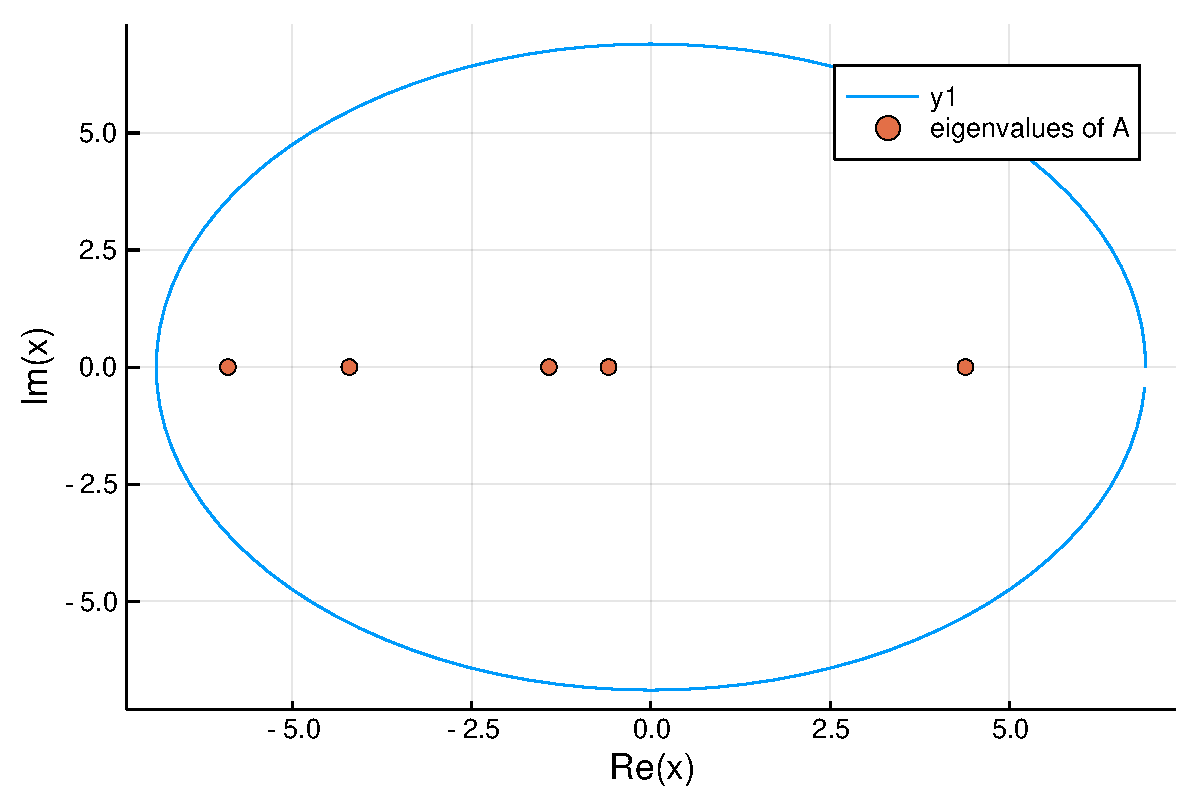
\includegraphics[width=\linewidth]{figures/Lecture9_2_1.pdf}

Here we wrap this up into a function \texttt{circle\_exp} that calculates the matrix exponential:


\begin{lstlisting}
(*@\HLJLk{function}@*) (*@\HLJLnf{circle{\_}exp}@*)(*@\HLJLp{(}@*)(*@\HLJLn{A}@*)(*@\HLJLp{,}@*) (*@\HLJLn{n}@*)(*@\HLJLp{,}@*) (*@\HLJLn{z\ensuremath{\_0}}@*)(*@\HLJLp{,}@*) (*@\HLJLn{r}@*)(*@\HLJLp{)}@*)
    (*@\HLJLn{z}@*)(*@\HLJLp{,}@*)(*@\HLJLn{w}@*) (*@\HLJLoB{=}@*) (*@\HLJLnf{circle{\_}rule}@*)(*@\HLJLp{(}@*)(*@\HLJLn{n}@*)(*@\HLJLp{,}@*)(*@\HLJLn{r}@*)(*@\HLJLp{)}@*)
    (*@\HLJLn{z}@*) (*@\HLJLoB{.+=}@*) (*@\HLJLn{z\ensuremath{\_0}}@*)

    (*@\HLJLn{ret}@*) (*@\HLJLoB{=}@*) (*@\HLJLnf{zero}@*)(*@\HLJLp{(}@*)(*@\HLJLn{A}@*)(*@\HLJLp{)}@*)
    (*@\HLJLk{for}@*) (*@\HLJLn{j}@*)(*@\HLJLoB{=}@*)(*@\HLJLni{1}@*)(*@\HLJLoB{:}@*)(*@\HLJLn{n}@*)
        (*@\HLJLn{ret}@*) (*@\HLJLoB{+=}@*) (*@\HLJLn{w}@*)(*@\HLJLp{[}@*)(*@\HLJLn{j}@*)(*@\HLJLp{]}@*)(*@\HLJLoB{*}@*)(*@\HLJLnf{exp}@*)(*@\HLJLp{(}@*)(*@\HLJLn{z}@*)(*@\HLJLp{[}@*)(*@\HLJLn{j}@*)(*@\HLJLp{])}@*)(*@\HLJLoB{*}@*)(*@\HLJLnf{inv}@*)(*@\HLJLp{(}@*)(*@\HLJLn{z}@*)(*@\HLJLp{[}@*)(*@\HLJLn{j}@*)(*@\HLJLp{]}@*)(*@\HLJLoB{*}@*)(*@\HLJLn{I}@*) (*@\HLJLoB{-}@*) (*@\HLJLn{A}@*)(*@\HLJLp{)}@*)
    (*@\HLJLk{end}@*)

    (*@\HLJLn{ret}@*)(*@\HLJLoB{/}@*)(*@\HLJLp{(}@*)(*@\HLJLni{2}@*)(*@\HLJLn{\ensuremath{\pi}}@*)(*@\HLJLoB{*}@*)(*@\HLJLn{im}@*)(*@\HLJLp{)}@*)
(*@\HLJLk{end}@*)
   
(*@\HLJLnf{circle{\_}exp}@*)(*@\HLJLp{(}@*)(*@\HLJLn{A}@*)(*@\HLJLp{,}@*) (*@\HLJLni{100}@*)(*@\HLJLp{,}@*) (*@\HLJLni{0}@*)(*@\HLJLp{,}@*) (*@\HLJLnfB{8.0}@*)(*@\HLJLp{)}@*) (*@\HLJLoB{-}@*)(*@\HLJLnf{exp}@*)(*@\HLJLp{(}@*)(*@\HLJLn{A}@*)(*@\HLJLp{)}@*) (*@\HLJLoB{|>}@*)(*@\HLJLn{norm}@*)
\end{lstlisting}

\begin{lstlisting}
1.0969975702206919e-12
\end{lstlisting}


In this case, it is beneficial to use an ellipse:


\begin{lstlisting}
(*@\HLJLk{function}@*) (*@\HLJLnf{ellipse{\_}rule}@*)(*@\HLJLp{(}@*)(*@\HLJLn{n}@*)(*@\HLJLp{,}@*) (*@\HLJLn{a}@*)(*@\HLJLp{,}@*) (*@\HLJLn{b}@*)(*@\HLJLp{)}@*) 
    (*@\HLJLn{\ensuremath{\theta}}@*) (*@\HLJLoB{=}@*) (*@\HLJLnf{periodic{\_}rule}@*)(*@\HLJLp{(}@*)(*@\HLJLn{n}@*)(*@\HLJLp{)[}@*)(*@\HLJLni{1}@*)(*@\HLJLp{]}@*)
    (*@\HLJLn{a}@*)(*@\HLJLoB{*}@*)(*@\HLJLn{cos}@*)(*@\HLJLoB{.}@*)(*@\HLJLp{(}@*)(*@\HLJLn{\ensuremath{\theta}}@*)(*@\HLJLp{)}@*) (*@\HLJLoB{+}@*) (*@\HLJLn{b}@*)(*@\HLJLoB{*}@*)(*@\HLJLn{im}@*)(*@\HLJLoB{*}@*)(*@\HLJLn{sin}@*)(*@\HLJLoB{.}@*)(*@\HLJLp{(}@*)(*@\HLJLn{\ensuremath{\theta}}@*)(*@\HLJLp{),}@*) (*@\HLJLni{2}@*)(*@\HLJLn{\ensuremath{\pi}}@*)(*@\HLJLoB{/}@*)(*@\HLJLn{n}@*)(*@\HLJLoB{*}@*)(*@\HLJLp{(}@*)(*@\HLJLoB{-}@*)(*@\HLJLn{a}@*)(*@\HLJLoB{*}@*)(*@\HLJLn{sin}@*)(*@\HLJLoB{.}@*)(*@\HLJLp{(}@*)(*@\HLJLn{\ensuremath{\theta}}@*)(*@\HLJLp{)}@*) (*@\HLJLoB{+}@*) (*@\HLJLn{im}@*)(*@\HLJLoB{*}@*)(*@\HLJLn{b}@*)(*@\HLJLoB{*}@*)(*@\HLJLn{cos}@*)(*@\HLJLoB{.}@*)(*@\HLJLp{(}@*)(*@\HLJLn{\ensuremath{\theta}}@*)(*@\HLJLp{))}@*)
(*@\HLJLk{end}@*)
(*@\HLJLk{function}@*) (*@\HLJLnf{ellipse{\_}exp}@*)(*@\HLJLp{(}@*)(*@\HLJLn{A}@*)(*@\HLJLp{,}@*) (*@\HLJLn{n}@*)(*@\HLJLp{,}@*) (*@\HLJLn{z\ensuremath{\_0}}@*)(*@\HLJLp{,}@*) (*@\HLJLn{a}@*)(*@\HLJLp{,}@*) (*@\HLJLn{b}@*)(*@\HLJLp{)}@*)
    (*@\HLJLn{z}@*)(*@\HLJLp{,}@*)(*@\HLJLn{w}@*) (*@\HLJLoB{=}@*) (*@\HLJLnf{ellipse{\_}rule}@*)(*@\HLJLp{(}@*)(*@\HLJLn{n}@*)(*@\HLJLp{,}@*)(*@\HLJLn{a}@*)(*@\HLJLp{,}@*)(*@\HLJLn{b}@*)(*@\HLJLp{)}@*)
    (*@\HLJLn{z}@*) (*@\HLJLoB{.+=}@*) (*@\HLJLn{z\ensuremath{\_0}}@*)

    (*@\HLJLn{ret}@*) (*@\HLJLoB{=}@*) (*@\HLJLnf{zero}@*)(*@\HLJLp{(}@*)(*@\HLJLn{A}@*)(*@\HLJLp{)}@*)
    (*@\HLJLk{for}@*) (*@\HLJLn{j}@*)(*@\HLJLoB{=}@*)(*@\HLJLni{1}@*)(*@\HLJLoB{:}@*)(*@\HLJLn{n}@*)
        (*@\HLJLn{ret}@*) (*@\HLJLoB{+=}@*) (*@\HLJLn{w}@*)(*@\HLJLp{[}@*)(*@\HLJLn{j}@*)(*@\HLJLp{]}@*)(*@\HLJLoB{*}@*)(*@\HLJLnf{exp}@*)(*@\HLJLp{(}@*)(*@\HLJLn{z}@*)(*@\HLJLp{[}@*)(*@\HLJLn{j}@*)(*@\HLJLp{])}@*)(*@\HLJLoB{*}@*)(*@\HLJLnf{inv}@*)(*@\HLJLp{(}@*)(*@\HLJLn{z}@*)(*@\HLJLp{[}@*)(*@\HLJLn{j}@*)(*@\HLJLp{]}@*)(*@\HLJLoB{*}@*)(*@\HLJLn{I}@*) (*@\HLJLoB{-}@*) (*@\HLJLn{A}@*)(*@\HLJLp{)}@*)
    (*@\HLJLk{end}@*)
    (*@\HLJLn{ret}@*)(*@\HLJLoB{/}@*)(*@\HLJLp{(}@*)(*@\HLJLni{2}@*)(*@\HLJLn{\ensuremath{\pi}}@*)(*@\HLJLoB{*}@*)(*@\HLJLn{im}@*)(*@\HLJLp{)}@*)
(*@\HLJLk{end}@*)

(*@\HLJLnf{ellipse{\_}exp}@*)(*@\HLJLp{(}@*)(*@\HLJLn{A}@*)(*@\HLJLp{,}@*) (*@\HLJLni{50}@*)(*@\HLJLp{,}@*) (*@\HLJLni{0}@*)(*@\HLJLp{,}@*) (*@\HLJLnfB{8.0}@*)(*@\HLJLp{,}@*) (*@\HLJLnfB{5.0}@*)(*@\HLJLp{)}@*) (*@\HLJLoB{-}@*)(*@\HLJLnf{exp}@*)(*@\HLJLp{(}@*)(*@\HLJLn{A}@*)(*@\HLJLp{)}@*) (*@\HLJLoB{|>}@*)(*@\HLJLn{norm}@*)
\end{lstlisting}

\begin{lstlisting}
8.301219305234686e-13
\end{lstlisting}


For matrices with large negative eigenvalues (For example, discretisations of the Laplacian), complex quadrature can lead to much better accuracy than Taylor series:


\begin{lstlisting}
(*@\HLJLk{function}@*) (*@\HLJLnf{taylor{\_}exp}@*)(*@\HLJLp{(}@*)(*@\HLJLn{A}@*)(*@\HLJLp{,}@*)(*@\HLJLn{n}@*)(*@\HLJLp{)}@*)
    (*@\HLJLn{ret}@*) (*@\HLJLoB{=}@*) (*@\HLJLnf{Matrix}@*)(*@\HLJLp{(}@*)(*@\HLJLn{I}@*)(*@\HLJLp{,}@*) (*@\HLJLnf{size}@*)(*@\HLJLp{(}@*)(*@\HLJLn{A}@*)(*@\HLJLp{))}@*)
    (*@\HLJLk{for}@*) (*@\HLJLn{k}@*)(*@\HLJLoB{=}@*)(*@\HLJLni{1}@*)(*@\HLJLoB{:}@*)(*@\HLJLn{n}@*)
        (*@\HLJLn{ret}@*) (*@\HLJLoB{+=}@*) (*@\HLJLn{A}@*)(*@\HLJLoB{{\textasciicircum}}@*)(*@\HLJLn{k}@*)(*@\HLJLoB{/}@*)(*@\HLJLnf{factorial}@*)(*@\HLJLp{(}@*)(*@\HLJLnfB{1.0}@*)(*@\HLJLn{k}@*)(*@\HLJLp{)}@*)
    (*@\HLJLk{end}@*)
    (*@\HLJLn{ret}@*)
(*@\HLJLk{end}@*)

(*@\HLJLn{B}@*) (*@\HLJLoB{=}@*) (*@\HLJLn{A}@*) (*@\HLJLoB{-}@*) (*@\HLJLni{20}@*)(*@\HLJLn{I}@*)

(*@\HLJLnf{taylor{\_}exp}@*)(*@\HLJLp{(}@*)(*@\HLJLn{B}@*)(*@\HLJLp{,}@*) (*@\HLJLni{200}@*)(*@\HLJLp{)}@*) (*@\HLJLoB{-}@*)(*@\HLJLnf{exp}@*)(*@\HLJLp{(}@*)(*@\HLJLn{B}@*)(*@\HLJLp{)}@*) (*@\HLJLoB{|>}@*)(*@\HLJLn{norm}@*)
\end{lstlisting}

\begin{lstlisting}
7.751291385269999e-6
\end{lstlisting}


We can use an ellpise to surround the spectrum:


\begin{lstlisting}
(*@\HLJLnf{scatter}@*)(*@\HLJLp{(}@*)(*@\HLJLn{complex}@*)(*@\HLJLoB{.}@*)(*@\HLJLp{(}@*)(*@\HLJLnf{eigvals}@*)(*@\HLJLp{(}@*)(*@\HLJLn{B}@*)(*@\HLJLp{)))}@*)
(*@\HLJLnf{plot!}@*)(*@\HLJLp{(}@*)(*@\HLJLnf{ellipse{\_}rule}@*)(*@\HLJLp{(}@*)(*@\HLJLni{50}@*)(*@\HLJLp{,}@*)(*@\HLJLni{8}@*)(*@\HLJLp{,}@*)(*@\HLJLni{5}@*)(*@\HLJLp{)[}@*)(*@\HLJLni{1}@*)(*@\HLJLp{]}@*) (*@\HLJLoB{.-}@*) (*@\HLJLni{20}@*)(*@\HLJLp{)}@*)

(*@\HLJLnf{norm}@*)(*@\HLJLp{(}@*)(*@\HLJLnf{ellipse{\_}exp}@*)(*@\HLJLp{(}@*)(*@\HLJLn{B}@*)(*@\HLJLp{,}@*) (*@\HLJLni{50}@*)(*@\HLJLp{,}@*) (*@\HLJLoB{-}@*)(*@\HLJLnfB{20.0}@*)(*@\HLJLp{,}@*) (*@\HLJLnfB{8.0}@*)(*@\HLJLp{,}@*) (*@\HLJLnfB{5.0}@*)(*@\HLJLp{)}@*) (*@\HLJLoB{-}@*) (*@\HLJLnf{exp}@*)(*@\HLJLp{(}@*)(*@\HLJLn{B}@*)(*@\HLJLp{))}@*)
\end{lstlisting}

\begin{lstlisting}
5.991775428348182e-22
\end{lstlisting}


\subsection{Finite differences and (fractional) heat equation}
As a first application we consider approximation of the solution of the heat equation $u(t,x)$, for $\Delta u := u_{xx}$ we have:

\[
u_t = \Delta u
\]
on $[0,1]$ with Dirichlet conditions $u(t,0) = u(t,1) = 0$ and initial condition $u(0,x) = u_0(x)$.  We approximate the solution by its values at a grid, that is, we have time dependent vector $\vc u(t)$  which we hope satisfies the property that at any time $t$

\[
\vc u(t) \approx \Vectt[u({t,x_1}), \dots, u({t,x_N})]
\]
where $x_j = j/(N+1)$ is an evenly spaced grid. Note we use that $u(t,x_0) = u(t,0) = 0$ and $u(t,x_{N+1}) = u(t,1) = 0$.

Recall from Taylor series that for a smooth enough function $f(x)$ we have 


\begin{align*}
{f(x+h) - 2 f(x) + f(x-h) \over h^2} &\approx {f(x) + f'(x) h + f''(x) h^2/2 - 2 f(x) + f(x) - f'(x) h + f''(x) h^2/2  \over h^2}\\
&= f''(x)
\end{align*}
For $h = 1/(N+1)$ this therefore gives


\begin{align*}
u_xx(t,x_1) & \approx {u(t,x_2) - 2 u(t,x_1) + u(t,x_0) \over h^2} = {u(t,x_2) - 2 u(t,x_1) \over h^2}  \\
u_xx(t,x_N) & \approx {u(t,x_{N+1}) - 2 u(t,x_N) + u(t,x_{N-1}) \over h^2} = { - 2 u(t,x_N) + u(t,x_{N-1}) \over h^2}  \\
u_xx(t,x_j) & \approx {u(t,x_{j+1}) - 2 u(t,x_j) + u(t,x_{j-1}) \over h^2}
\end{align*}
Or in vector form we have

\[
\Vectt[{u_xx(t,x_1)}, \dots, {u_xx(t,x_N)}] \approx \Delta \Vectt[{u(t,x_1)}, \dots, {u(t,x_N)}]
\]
where 

\[
\Delta_N = {1 \over h^2} \sopmatrix{-2 & 1 \\ 1 & -2 & 1 \\ & \ddots & \ddots & \ddots \\ && 1 & -2 & 1 \\ &&&1 &-2 }
\]
In short: a natural approximation to the heat equation is

\[
\vc u'(t) = \Delta_N \vc u(t), \qquad u(0) = \vc u_0
\]
where $\vc u_0 = \vectt[u_0(x_1), \dots, u_0(x_N)]$. Thus to evaluate the solution at time $t$ we have

\[
\vc u(t) = \E^{\Delta_N t} \vc u_0 \approx {1 \over 2\pi \I} \oint_\gamma \E^{\zeta t} (\zeta I - \Delta_N)^{-1} \vc u_0 \D \zeta.
\]
We need to surround the spectrum of $\Delta_N$. In this case it suffices to use Gershgorin's theorem to determine:

\[
\sigma(\Delta_N) \subset [-4/h^2,0] = [-4 (N+1)^2,0]
\]
Now for something more complicated, the fractional heat equation:

\[
u_t = - (-\Delta)^\alpha u
\]
where $\alpha$ is say $1/2$. These come up in applications involving "memory", for example, in medical imaging where  tissue changes over time. They also come up in Levy flights, that is, stochastic differential equations with heavy-tailed  distributions. The precise definition is beyond the scope of this course, but in terms of numerical approximation it is natural to discretise as

\[
\vc u'(t) = - (-\Delta_N)^\alpha \vc u
\]
Or in other words,

\[
\vc u(t) = \E^{-(-\Delta_N)^\alpha t} \vc u_0 \approx {1 \over 2\pi \I} \oint_\gamma \E^{-\zeta^\alpha t} (\zeta I + \Delta_N)^{-1}  \vc u_0 \D \zeta.
\]
Gershgorin's theorem does not help us: it states 

\[
\sigma(-\Delta_N) \subset [0,4/h^2]
\]
but $\E^{- \zeta^\alpha t }$ has a branch cut right at 0. Fortunately in this case we have more understanding of the spectrum of $\Delta_N$. In  particular, for 

\[
J = \sopmatrix{0 & 1 \\ 1 & 0 & 1 \\ & \ddots & \ddots & \ddots \\ && 1 & 0 & 1 \\ &&& 1 & 0}
\]
we have from trigonometric relationships 

\[
2\cos \theta \sin k \theta = \sin (k+1) \theta + \sin(k-1) \theta
\]
that


\begin{align*}
J \Vectt[\sin \theta, \sin 2 \theta , \dots, \sin N \theta] = \Vectt[\sin 2 \theta, \sin 3 \theta + \sin \theta ,\dots, \sin(N-2) \theta + \sin N \theta, \sin (N-1) \theta ]\\
&= 2 \cos \theta\Vectt[\sin \theta, \sin 2 \theta , \dots, \sin (N-1) \theta,\sin N \theta] - \Vectt[0,0,\dots,0,\sin (N+1) \theta]
\end{align*}
The second term is zero when $\theta = \theta_j = j \pi / (N+1)$, thus we know the eigenvalues of $\Delta$ are $\lambda_j = 2 \cos \theta_j$ for $j = 1,\ldots,N$. ($j = 0$ is not valid as then the "eigenvector" would be zero.) We need to bound the spectrum away from $0$ and $2$. First note from telescoping properties of cosine Taylor series we have

\[
\cos x = 1 - x^2/2  + x^4/24 - \cdots \leq 1 - x^2/2 + x^4/24
\]
thus our bound above is

\[
2 \cos \theta_1 = 2 \cos {\pi  \over N+1} \leq 2 - \pr({\pi \over N+1})^2 + \pr({\pi \over N+1})^4/12
\]
The same holds for the bound below:

\[
2 \cos \theta_N \geq -2 + \pr({\pi \over N+1})^2 - {\pi^4 \over 12 (N+1)^2}
\]
Thus we have

\[
\sigma(\Delta_N) = \sigma(J - 2I)/h^2 \subset \br[-4 (N+1)^2 + \pi^2 - {\pi^4 \over 12 (N+1)^2},-\pi^2 + {\pi^4 \over 12 (N+1)^2}]
\]
Thus it suffices to take an ellipse contour passing through say $\pi^2/2$ and $-4 (N+1)^2$.

\textbf{Demonstration} We first demonstrate using the built-in matrix exponential. We can construct $\Delta$ as follows:


\begin{lstlisting}
(*@\HLJLn{N}@*) (*@\HLJLoB{=}@*) (*@\HLJLni{20}@*)
(*@\HLJLn{h}@*) (*@\HLJLoB{=}@*) (*@\HLJLni{1}@*)(*@\HLJLoB{/}@*)(*@\HLJLn{N}@*)
(*@\HLJLn{\ensuremath{\Delta}}@*) (*@\HLJLoB{=}@*) (*@\HLJLnf{SymTridiagonal}@*)(*@\HLJLp{(}@*)(*@\HLJLnf{fill}@*)(*@\HLJLp{(}@*)(*@\HLJLoB{-}@*)(*@\HLJLni{2}@*)(*@\HLJLp{,}@*)(*@\HLJLn{N}@*)(*@\HLJLp{),}@*) (*@\HLJLnf{fill}@*)(*@\HLJLp{(}@*)(*@\HLJLni{1}@*)(*@\HLJLp{,}@*)(*@\HLJLn{N}@*)(*@\HLJLoB{-}@*)(*@\HLJLni{1}@*)(*@\HLJLp{))}@*)(*@\HLJLoB{/}@*)(*@\HLJLn{h}@*)(*@\HLJLoB{{\textasciicircum}}@*)(*@\HLJLni{2}@*)
\end{lstlisting}

\begin{lstlisting}
20(*@\ensuremath{\times}@*)20 SymTridiagonal{Float64,Array{Float64,1}}:
 -800.0   400.0      (*@\ensuremath{\cdot}@*)       (*@\ensuremath{\cdot}@*)       (*@\ensuremath{\cdot}@*)   (*@\ensuremath{\dots}@*)      (*@\ensuremath{\cdot}@*)       (*@\ensuremath{\cdot}@*)       (*@\ensuremath{\cdot}@*)       (*@\ensuremath{\cdot}@*) 
  400.0  -800.0   400.0      (*@\ensuremath{\cdot}@*)       (*@\ensuremath{\cdot}@*)          (*@\ensuremath{\cdot}@*)       (*@\ensuremath{\cdot}@*)       (*@\ensuremath{\cdot}@*)       (*@\ensuremath{\cdot}@*) 
     (*@\ensuremath{\cdot}@*)    400.0  -800.0   400.0      (*@\ensuremath{\cdot}@*)          (*@\ensuremath{\cdot}@*)       (*@\ensuremath{\cdot}@*)       (*@\ensuremath{\cdot}@*)       (*@\ensuremath{\cdot}@*) 
     (*@\ensuremath{\cdot}@*)       (*@\ensuremath{\cdot}@*)    400.0  -800.0   400.0         (*@\ensuremath{\cdot}@*)       (*@\ensuremath{\cdot}@*)       (*@\ensuremath{\cdot}@*)       (*@\ensuremath{\cdot}@*) 
     (*@\ensuremath{\cdot}@*)       (*@\ensuremath{\cdot}@*)       (*@\ensuremath{\cdot}@*)    400.0  -800.0         (*@\ensuremath{\cdot}@*)       (*@\ensuremath{\cdot}@*)       (*@\ensuremath{\cdot}@*)       (*@\ensuremath{\cdot}@*) 
     (*@\ensuremath{\cdot}@*)       (*@\ensuremath{\cdot}@*)       (*@\ensuremath{\cdot}@*)       (*@\ensuremath{\cdot}@*)    400.0  (*@\ensuremath{\dots}@*)      (*@\ensuremath{\cdot}@*)       (*@\ensuremath{\cdot}@*)       (*@\ensuremath{\cdot}@*)       (*@\ensuremath{\cdot}@*) 
     (*@\ensuremath{\cdot}@*)       (*@\ensuremath{\cdot}@*)       (*@\ensuremath{\cdot}@*)       (*@\ensuremath{\cdot}@*)       (*@\ensuremath{\cdot}@*)          (*@\ensuremath{\cdot}@*)       (*@\ensuremath{\cdot}@*)       (*@\ensuremath{\cdot}@*)       (*@\ensuremath{\cdot}@*) 
     (*@\ensuremath{\cdot}@*)       (*@\ensuremath{\cdot}@*)       (*@\ensuremath{\cdot}@*)       (*@\ensuremath{\cdot}@*)       (*@\ensuremath{\cdot}@*)          (*@\ensuremath{\cdot}@*)       (*@\ensuremath{\cdot}@*)       (*@\ensuremath{\cdot}@*)       (*@\ensuremath{\cdot}@*) 
     (*@\ensuremath{\cdot}@*)       (*@\ensuremath{\cdot}@*)       (*@\ensuremath{\cdot}@*)       (*@\ensuremath{\cdot}@*)       (*@\ensuremath{\cdot}@*)          (*@\ensuremath{\cdot}@*)       (*@\ensuremath{\cdot}@*)       (*@\ensuremath{\cdot}@*)       (*@\ensuremath{\cdot}@*) 
     (*@\ensuremath{\cdot}@*)       (*@\ensuremath{\cdot}@*)       (*@\ensuremath{\cdot}@*)       (*@\ensuremath{\cdot}@*)       (*@\ensuremath{\cdot}@*)          (*@\ensuremath{\cdot}@*)       (*@\ensuremath{\cdot}@*)       (*@\ensuremath{\cdot}@*)       (*@\ensuremath{\cdot}@*) 
     (*@\ensuremath{\cdot}@*)       (*@\ensuremath{\cdot}@*)       (*@\ensuremath{\cdot}@*)       (*@\ensuremath{\cdot}@*)       (*@\ensuremath{\cdot}@*)   (*@\ensuremath{\dots}@*)      (*@\ensuremath{\cdot}@*)       (*@\ensuremath{\cdot}@*)       (*@\ensuremath{\cdot}@*)       (*@\ensuremath{\cdot}@*) 
     (*@\ensuremath{\cdot}@*)       (*@\ensuremath{\cdot}@*)       (*@\ensuremath{\cdot}@*)       (*@\ensuremath{\cdot}@*)       (*@\ensuremath{\cdot}@*)          (*@\ensuremath{\cdot}@*)       (*@\ensuremath{\cdot}@*)       (*@\ensuremath{\cdot}@*)       (*@\ensuremath{\cdot}@*) 
     (*@\ensuremath{\cdot}@*)       (*@\ensuremath{\cdot}@*)       (*@\ensuremath{\cdot}@*)       (*@\ensuremath{\cdot}@*)       (*@\ensuremath{\cdot}@*)          (*@\ensuremath{\cdot}@*)       (*@\ensuremath{\cdot}@*)       (*@\ensuremath{\cdot}@*)       (*@\ensuremath{\cdot}@*) 
     (*@\ensuremath{\cdot}@*)       (*@\ensuremath{\cdot}@*)       (*@\ensuremath{\cdot}@*)       (*@\ensuremath{\cdot}@*)       (*@\ensuremath{\cdot}@*)          (*@\ensuremath{\cdot}@*)       (*@\ensuremath{\cdot}@*)       (*@\ensuremath{\cdot}@*)       (*@\ensuremath{\cdot}@*) 
     (*@\ensuremath{\cdot}@*)       (*@\ensuremath{\cdot}@*)       (*@\ensuremath{\cdot}@*)       (*@\ensuremath{\cdot}@*)       (*@\ensuremath{\cdot}@*)          (*@\ensuremath{\cdot}@*)       (*@\ensuremath{\cdot}@*)       (*@\ensuremath{\cdot}@*)       (*@\ensuremath{\cdot}@*) 
     (*@\ensuremath{\cdot}@*)       (*@\ensuremath{\cdot}@*)       (*@\ensuremath{\cdot}@*)       (*@\ensuremath{\cdot}@*)       (*@\ensuremath{\cdot}@*)   (*@\ensuremath{\dots}@*)   400.0      (*@\ensuremath{\cdot}@*)       (*@\ensuremath{\cdot}@*)       (*@\ensuremath{\cdot}@*) 
     (*@\ensuremath{\cdot}@*)       (*@\ensuremath{\cdot}@*)       (*@\ensuremath{\cdot}@*)       (*@\ensuremath{\cdot}@*)       (*@\ensuremath{\cdot}@*)      -800.0   400.0      (*@\ensuremath{\cdot}@*)       (*@\ensuremath{\cdot}@*) 
     (*@\ensuremath{\cdot}@*)       (*@\ensuremath{\cdot}@*)       (*@\ensuremath{\cdot}@*)       (*@\ensuremath{\cdot}@*)       (*@\ensuremath{\cdot}@*)       400.0  -800.0   400.0      (*@\ensuremath{\cdot}@*) 
     (*@\ensuremath{\cdot}@*)       (*@\ensuremath{\cdot}@*)       (*@\ensuremath{\cdot}@*)       (*@\ensuremath{\cdot}@*)       (*@\ensuremath{\cdot}@*)          (*@\ensuremath{\cdot}@*)    400.0  -800.0   400.0
     (*@\ensuremath{\cdot}@*)       (*@\ensuremath{\cdot}@*)       (*@\ensuremath{\cdot}@*)       (*@\ensuremath{\cdot}@*)       (*@\ensuremath{\cdot}@*)          (*@\ensuremath{\cdot}@*)       (*@\ensuremath{\cdot}@*)    400.0  -800.0
\end{lstlisting}


The solution with an initial condition $u_0(x) = x (1-x) \E^x$ is then:


\begin{lstlisting}
(*@\HLJLn{u0}@*) (*@\HLJLoB{=}@*) (*@\HLJLn{x}@*) (*@\HLJLoB{->}@*) (*@\HLJLn{x}@*) (*@\HLJLoB{*}@*) (*@\HLJLp{(}@*)(*@\HLJLni{1}@*)(*@\HLJLoB{-}@*)(*@\HLJLn{x}@*)(*@\HLJLp{)}@*) (*@\HLJLoB{*}@*) (*@\HLJLnf{exp}@*)(*@\HLJLp{(}@*)(*@\HLJLn{x}@*)(*@\HLJLp{)}@*)

(*@\HLJLn{xx}@*) (*@\HLJLoB{=}@*) (*@\HLJLnf{range}@*)(*@\HLJLp{(}@*)(*@\HLJLni{0}@*)(*@\HLJLp{,}@*)(*@\HLJLni{1}@*)(*@\HLJLp{;}@*) (*@\HLJLn{length}@*)(*@\HLJLoB{=}@*)(*@\HLJLn{N}@*)(*@\HLJLoB{+}@*)(*@\HLJLni{2}@*)(*@\HLJLp{)}@*)
(*@\HLJLn{A}@*) (*@\HLJLoB{=}@*) (*@\HLJLnf{Matrix}@*)(*@\HLJLp{(}@*)(*@\HLJLn{\ensuremath{\Delta}}@*)(*@\HLJLp{)}@*) (*@\HLJLcs{{\#}}@*) (*@\HLJLcs{Need}@*) (*@\HLJLcs{to}@*) (*@\HLJLcs{convert}@*) (*@\HLJLcs{to}@*) (*@\HLJLcs{dense}@*) (*@\HLJLcs{matrix}@*) (*@\HLJLcs{to}@*) (*@\HLJLcs{diagonalise}@*)
(*@\HLJLn{p}@*) (*@\HLJLoB{=}@*) (*@\HLJLnf{plot}@*)(*@\HLJLp{()}@*)
(*@\HLJLk{for}@*) (*@\HLJLn{t}@*) (*@\HLJLkp{in}@*) (*@\HLJLni{0}@*)(*@\HLJLoB{:}@*)(*@\HLJLnfB{0.1}@*)(*@\HLJLoB{:}@*)(*@\HLJLnfB{0.5}@*)
    (*@\HLJLnf{plot!}@*)(*@\HLJLp{(}@*)(*@\HLJLn{xx}@*)(*@\HLJLp{,}@*) (*@\HLJLp{[}@*)(*@\HLJLni{0}@*)(*@\HLJLp{;}@*) (*@\HLJLnf{exp}@*)(*@\HLJLp{(}@*)(*@\HLJLn{A}@*)(*@\HLJLoB{*}@*)(*@\HLJLn{t}@*)(*@\HLJLp{)}@*)(*@\HLJLoB{*}@*)(*@\HLJLn{u0}@*)(*@\HLJLoB{.}@*)(*@\HLJLp{(}@*)(*@\HLJLn{xx}@*)(*@\HLJLp{[}@*)(*@\HLJLni{2}@*)(*@\HLJLoB{:}@*)(*@\HLJLk{end}@*)(*@\HLJLoB{-}@*)(*@\HLJLni{1}@*)(*@\HLJLp{]);}@*) (*@\HLJLni{0}@*)(*@\HLJLp{];}@*) (*@\HLJLn{label}@*)(*@\HLJLoB{=}@*)(*@\HLJLs{"{}t}@*) (*@\HLJLs{=}@*) (*@\HLJLsi{{\$}t}@*)(*@\HLJLs{"{}}@*)(*@\HLJLp{)}@*)
(*@\HLJLk{end}@*)
(*@\HLJLn{p}@*)
\end{lstlisting}

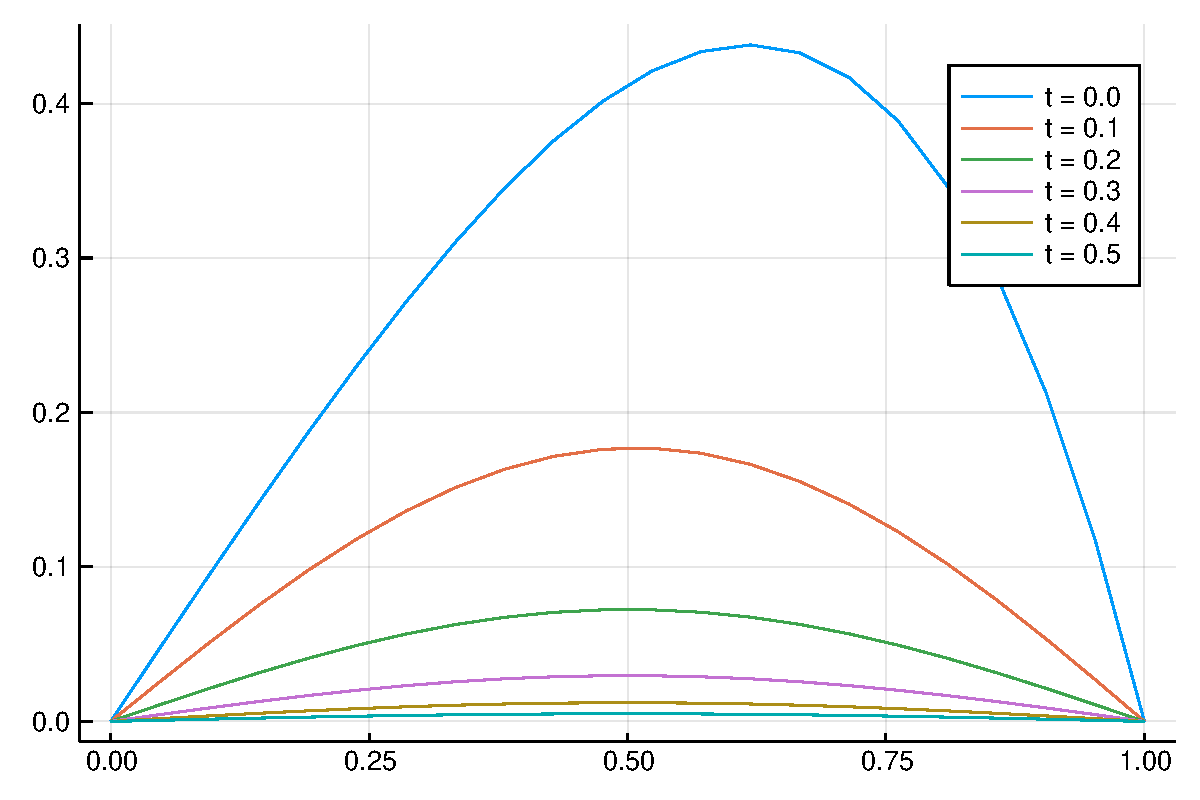
\includegraphics[width=\linewidth]{figures/Lecture9_8_1.pdf}

The above calculation is expensive: it does not take into account the sparsity of \texttt{\ensuremath{\Delta}}. To do  better we use Cauchy's integral formula with trapezium rule. First design an ellipse that surrounds the spectrum:


\begin{lstlisting}
(*@\HLJLn{m}@*) (*@\HLJLoB{=}@*) (*@\HLJLni{20{\_}000}@*)
(*@\HLJLn{z}@*)(*@\HLJLp{,}@*)(*@\HLJLn{w}@*) (*@\HLJLoB{=}@*) (*@\HLJLnf{ellipse{\_}rule}@*)(*@\HLJLp{(}@*)(*@\HLJLn{m}@*)(*@\HLJLp{,}@*)(*@\HLJLni{2}@*)(*@\HLJLoB{/}@*)(*@\HLJLn{h}@*)(*@\HLJLoB{{\textasciicircum}}@*)(*@\HLJLni{2}@*)(*@\HLJLp{,}@*)(*@\HLJLni{1}@*)(*@\HLJLp{)}@*)
(*@\HLJLn{z}@*) (*@\HLJLoB{.-=}@*) (*@\HLJLni{2}@*)(*@\HLJLoB{/}@*)(*@\HLJLn{h}@*)(*@\HLJLoB{{\textasciicircum}}@*)(*@\HLJLni{2}@*) (*@\HLJLcs{{\#}}@*) (*@\HLJLcs{shift}@*) (*@\HLJLcs{to}@*) (*@\HLJLcs{negative}@*)
(*@\HLJLnf{plot}@*)(*@\HLJLp{(}@*)(*@\HLJLn{z}@*)(*@\HLJLp{;}@*) (*@\HLJLn{label}@*)(*@\HLJLoB{=}@*)(*@\HLJLs{"{}contour"{}}@*)(*@\HLJLp{)}@*)
(*@\HLJLnf{scatter!}@*)(*@\HLJLp{(}@*)(*@\HLJLnf{eigvals}@*)(*@\HLJLp{(}@*)(*@\HLJLn{\ensuremath{\Delta}}@*)(*@\HLJLp{),}@*) (*@\HLJLnf{zeros}@*)(*@\HLJLp{(}@*)(*@\HLJLn{N}@*)(*@\HLJLp{);}@*) (*@\HLJLn{markersize}@*)(*@\HLJLoB{=}@*)(*@\HLJLnfB{0.5}@*)(*@\HLJLp{,}@*) (*@\HLJLn{label}@*)(*@\HLJLoB{=}@*)(*@\HLJLs{"{}eigenvalues"{}}@*)(*@\HLJLp{)}@*)
\end{lstlisting}

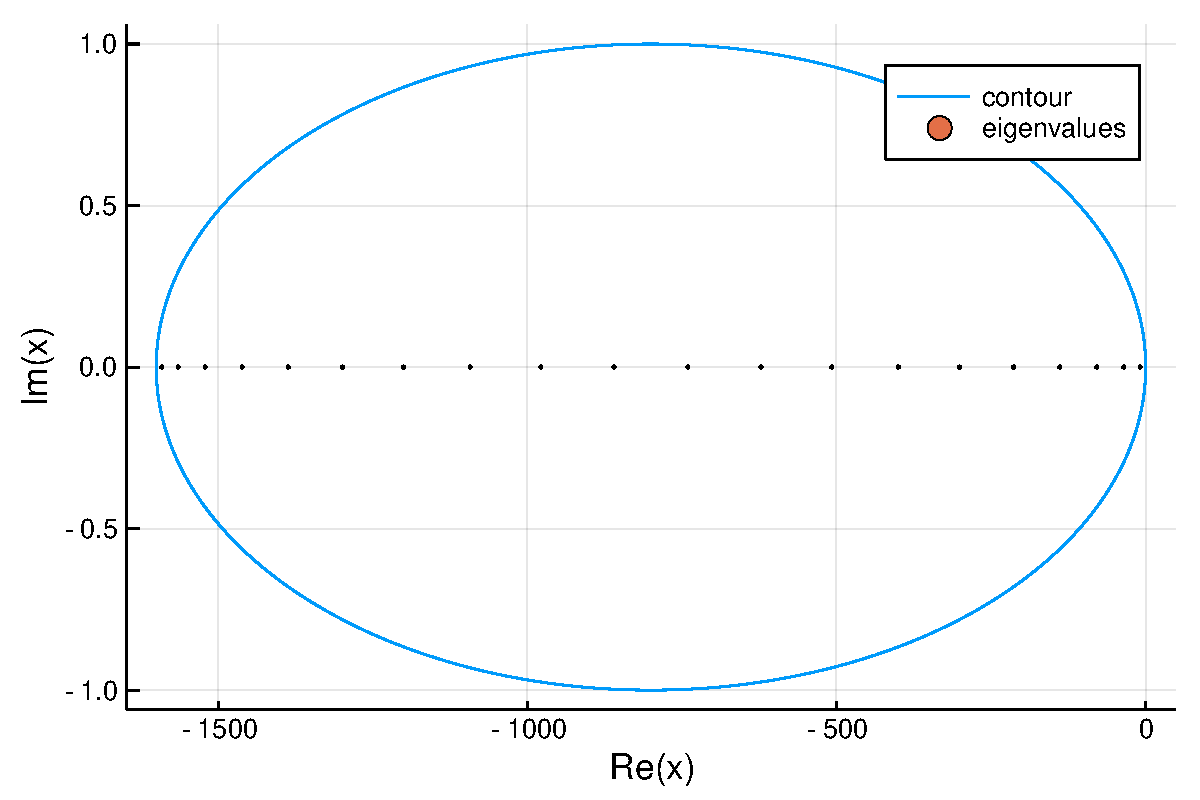
\includegraphics[width=\linewidth]{figures/Lecture9_9_1.pdf}

We thus can evaluate the matrix exponential at time $t$ using the quadrature rule:


\begin{lstlisting}
(*@\HLJLn{u0{\_}v}@*) (*@\HLJLoB{=}@*) (*@\HLJLn{u0}@*)(*@\HLJLoB{.}@*)(*@\HLJLp{(}@*)(*@\HLJLn{xx}@*)(*@\HLJLp{[}@*)(*@\HLJLni{2}@*)(*@\HLJLoB{:}@*)(*@\HLJLk{end}@*)(*@\HLJLoB{-}@*)(*@\HLJLni{1}@*)(*@\HLJLp{])}@*)
(*@\HLJLn{ret}@*) (*@\HLJLoB{=}@*) (*@\HLJLnf{zero}@*)(*@\HLJLp{(}@*)(*@\HLJLnf{complex}@*)(*@\HLJLp{(}@*)(*@\HLJLn{u0{\_}v}@*)(*@\HLJLp{))}@*)
(*@\HLJLn{t}@*) (*@\HLJLoB{=}@*) (*@\HLJLnfB{0.5}@*)
(*@\HLJLk{for}@*) (*@\HLJLn{j}@*)(*@\HLJLoB{=}@*)(*@\HLJLni{1}@*)(*@\HLJLoB{:}@*)(*@\HLJLnf{length}@*)(*@\HLJLp{(}@*)(*@\HLJLn{z}@*)(*@\HLJLp{)}@*)
    (*@\HLJLkd{global}@*) (*@\HLJLn{ret}@*)(*@\HLJLp{,}@*) (*@\HLJLn{w}@*)(*@\HLJLp{,}@*) (*@\HLJLn{z}@*)
    (*@\HLJLn{ret}@*) (*@\HLJLoB{+=}@*) (*@\HLJLn{w}@*)(*@\HLJLp{[}@*)(*@\HLJLn{j}@*)(*@\HLJLp{]}@*)(*@\HLJLoB{*}@*)(*@\HLJLnf{exp}@*)(*@\HLJLp{(}@*)(*@\HLJLn{t}@*)(*@\HLJLoB{*}@*)(*@\HLJLn{z}@*)(*@\HLJLp{[}@*)(*@\HLJLn{j}@*)(*@\HLJLp{])}@*) (*@\HLJLoB{*}@*) (*@\HLJLp{((}@*)(*@\HLJLn{z}@*)(*@\HLJLp{[}@*)(*@\HLJLn{j}@*)(*@\HLJLp{]}@*)(*@\HLJLoB{*}@*)(*@\HLJLn{I}@*) (*@\HLJLoB{-}@*) (*@\HLJLn{\ensuremath{\Delta}}@*)(*@\HLJLp{)}@*) (*@\HLJLoB{{\textbackslash}}@*) (*@\HLJLn{u0{\_}v}@*)(*@\HLJLp{)}@*)
(*@\HLJLk{end}@*)
(*@\HLJLnf{norm}@*)(*@\HLJLp{(}@*)(*@\HLJLn{ret}@*)(*@\HLJLoB{/}@*)(*@\HLJLp{(}@*)(*@\HLJLni{2}@*)(*@\HLJLn{\ensuremath{\pi}}@*)(*@\HLJLoB{*}@*)(*@\HLJLn{im}@*)(*@\HLJLp{)}@*) (*@\HLJLoB{-}@*) (*@\HLJLnf{exp}@*)(*@\HLJLp{(}@*)(*@\HLJLn{A}@*)(*@\HLJLoB{*}@*)(*@\HLJLn{t}@*)(*@\HLJLp{)}@*)(*@\HLJLoB{*}@*)(*@\HLJLn{u0{\_}v}@*)(*@\HLJLp{)}@*) (*@\HLJLcs{{\#}}@*) (*@\HLJLcs{matches}@*) (*@\HLJLcs{to}@*) (*@\HLJLcs{high}@*) (*@\HLJLcs{accuracy}@*)
\end{lstlisting}

\begin{lstlisting}
2.058538199502512e-13
\end{lstlisting}


For fractional heat equation, we have slower diffusion:


\begin{lstlisting}
(*@\HLJLn{A}@*) (*@\HLJLoB{=}@*) (*@\HLJLoB{-}@*)(*@\HLJLnf{sqrt}@*)(*@\HLJLp{(}@*)(*@\HLJLoB{-}@*)(*@\HLJLnf{Matrix}@*)(*@\HLJLp{(}@*)(*@\HLJLn{\ensuremath{\Delta}}@*)(*@\HLJLp{))}@*)
(*@\HLJLn{p}@*) (*@\HLJLoB{=}@*) (*@\HLJLnf{plot}@*)(*@\HLJLp{()}@*)
(*@\HLJLk{for}@*) (*@\HLJLn{t}@*) (*@\HLJLkp{in}@*) (*@\HLJLni{0}@*)(*@\HLJLoB{:}@*)(*@\HLJLnfB{0.1}@*)(*@\HLJLoB{:}@*)(*@\HLJLnfB{0.5}@*)
    (*@\HLJLnf{plot!}@*)(*@\HLJLp{(}@*)(*@\HLJLn{xx}@*)(*@\HLJLp{,}@*) (*@\HLJLp{[}@*)(*@\HLJLni{0}@*)(*@\HLJLp{;}@*) (*@\HLJLnf{exp}@*)(*@\HLJLp{(}@*)(*@\HLJLn{A}@*)(*@\HLJLoB{*}@*)(*@\HLJLn{t}@*)(*@\HLJLp{)}@*)(*@\HLJLoB{*}@*)(*@\HLJLn{u0}@*)(*@\HLJLoB{.}@*)(*@\HLJLp{(}@*)(*@\HLJLn{xx}@*)(*@\HLJLp{[}@*)(*@\HLJLni{2}@*)(*@\HLJLoB{:}@*)(*@\HLJLk{end}@*)(*@\HLJLoB{-}@*)(*@\HLJLni{1}@*)(*@\HLJLp{]);}@*) (*@\HLJLni{0}@*)(*@\HLJLp{];}@*) (*@\HLJLn{label}@*)(*@\HLJLoB{=}@*)(*@\HLJLs{"{}t}@*) (*@\HLJLs{=}@*) (*@\HLJLsi{{\$}t}@*)(*@\HLJLs{"{}}@*)(*@\HLJLp{)}@*)
(*@\HLJLk{end}@*)
(*@\HLJLn{p}@*)
\end{lstlisting}

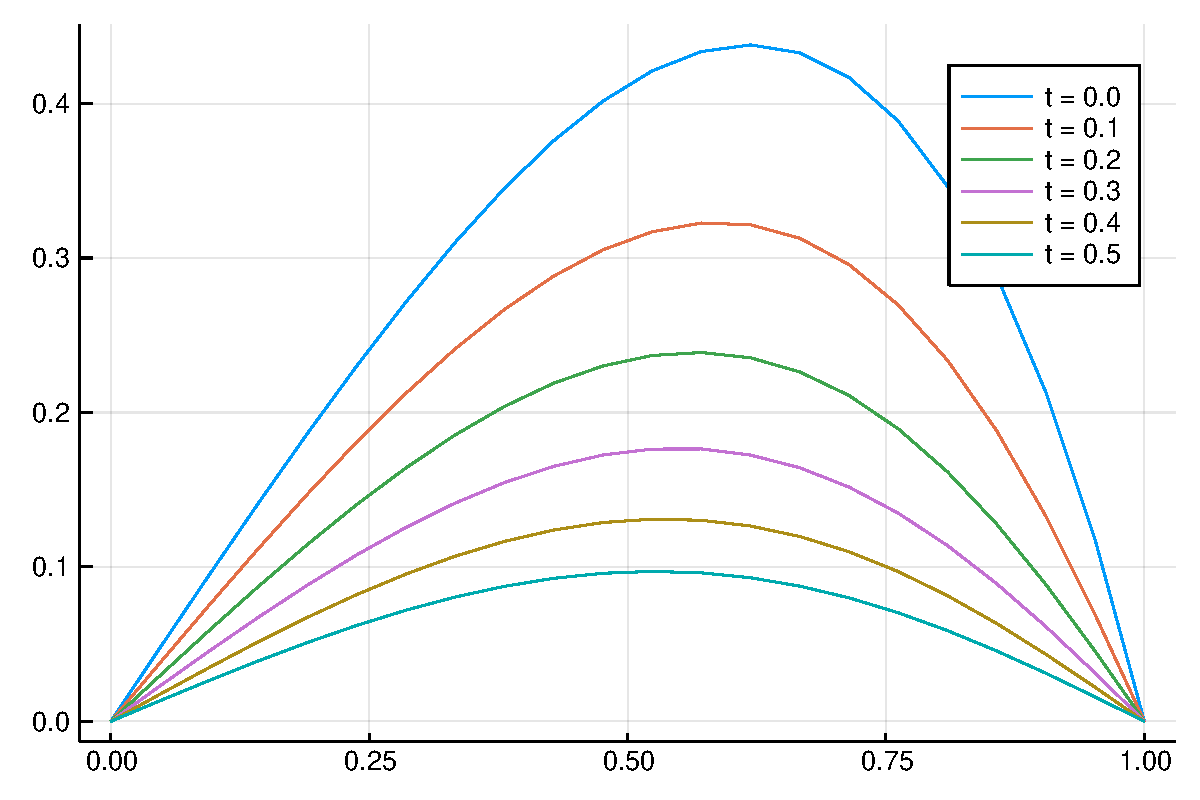
\includegraphics[width=\linewidth]{figures/Lecture9_11_1.pdf}

We need to be more careful and navigate the branch cut of $\E^{-\sqrt{z}}$. That is, we need the following contour (note we evaluate on $-\Delta$):


\begin{lstlisting}
(*@\HLJLn{m}@*) (*@\HLJLoB{=}@*) (*@\HLJLni{20{\_}000}@*)
(*@\HLJLn{z}@*)(*@\HLJLp{,}@*)(*@\HLJLn{w}@*) (*@\HLJLoB{=}@*) (*@\HLJLnf{ellipse{\_}rule}@*)(*@\HLJLp{(}@*)(*@\HLJLn{m}@*)(*@\HLJLp{,}@*)(*@\HLJLni{2}@*)(*@\HLJLoB{/}@*)(*@\HLJLn{h}@*)(*@\HLJLoB{{\textasciicircum}}@*)(*@\HLJLni{2}@*)(*@\HLJLp{,}@*)(*@\HLJLni{1}@*)(*@\HLJLp{)}@*)
(*@\HLJLn{z}@*) (*@\HLJLoB{.+=}@*) (*@\HLJLni{2}@*)(*@\HLJLoB{/}@*)(*@\HLJLn{h}@*)(*@\HLJLoB{{\textasciicircum}}@*)(*@\HLJLni{2}@*) (*@\HLJLoB{+}@*) (*@\HLJLn{\ensuremath{\pi}}@*)(*@\HLJLoB{{\textasciicircum}}@*)(*@\HLJLni{2}@*)(*@\HLJLoB{/}@*)(*@\HLJLni{2}@*) (*@\HLJLcs{{\#}}@*) (*@\HLJLcs{shift}@*) (*@\HLJLcs{to}@*) (*@\HLJLcs{positive}@*)
(*@\HLJLnf{plot}@*)(*@\HLJLp{(}@*)(*@\HLJLn{z}@*)(*@\HLJLp{;}@*) (*@\HLJLn{label}@*)(*@\HLJLoB{=}@*)(*@\HLJLs{"{}contour"{}}@*)(*@\HLJLp{)}@*)
(*@\HLJLnf{scatter!}@*)(*@\HLJLp{(}@*)(*@\HLJLnf{eigvals}@*)(*@\HLJLp{(}@*)(*@\HLJLoB{-}@*)(*@\HLJLn{\ensuremath{\Delta}}@*)(*@\HLJLp{),}@*) (*@\HLJLnf{zeros}@*)(*@\HLJLp{(}@*)(*@\HLJLn{N}@*)(*@\HLJLp{);}@*) (*@\HLJLn{markersize}@*)(*@\HLJLoB{=}@*)(*@\HLJLnfB{0.5}@*)(*@\HLJLp{,}@*) (*@\HLJLn{label}@*)(*@\HLJLoB{=}@*)(*@\HLJLs{"{}eigenvalues"{}}@*)(*@\HLJLp{)}@*)
(*@\HLJLnf{plot!}@*)(*@\HLJLp{([}@*)(*@\HLJLoB{-}@*)(*@\HLJLni{2000}@*)(*@\HLJLp{,}@*)(*@\HLJLni{0}@*)(*@\HLJLp{],[}@*)(*@\HLJLni{0}@*)(*@\HLJLp{,}@*)(*@\HLJLni{0}@*)(*@\HLJLp{];}@*) (*@\HLJLn{label}@*)(*@\HLJLoB{=}@*)(*@\HLJLs{"{}branch}@*) (*@\HLJLs{cut"{}}@*)(*@\HLJLp{)}@*)
\end{lstlisting}

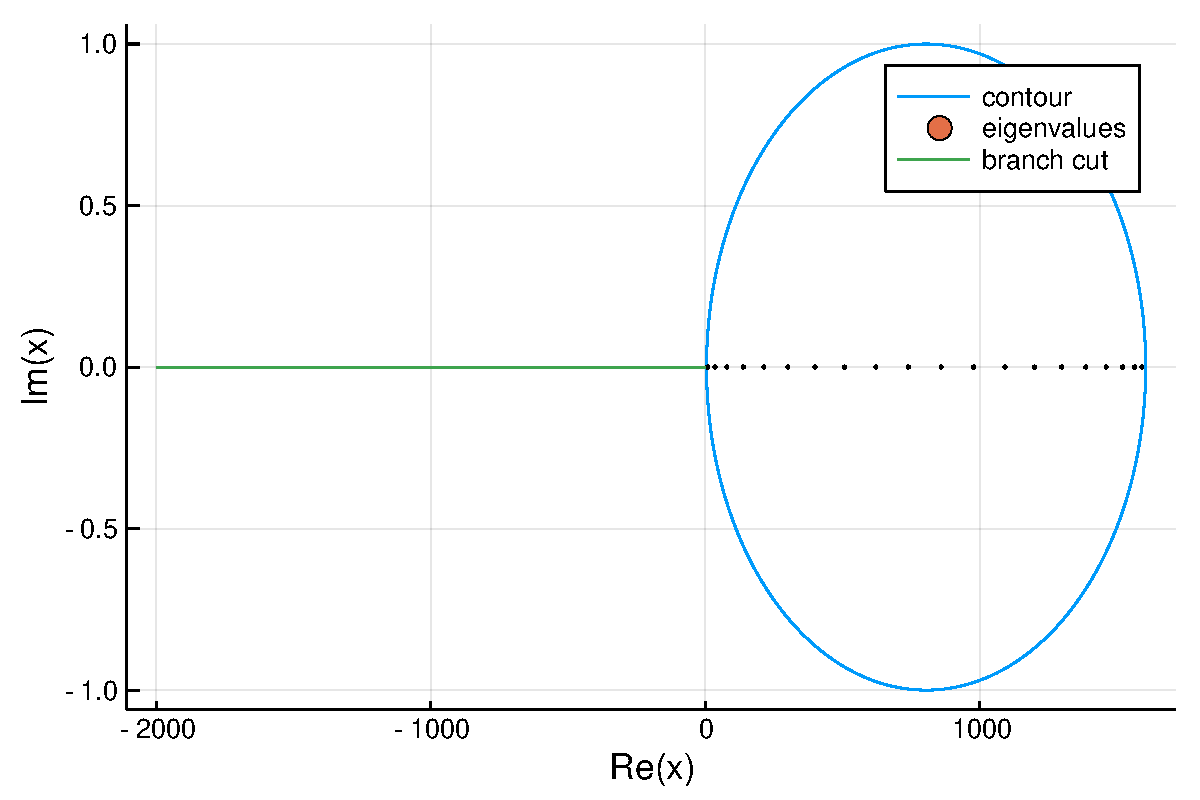
\includegraphics[width=\linewidth]{figures/Lecture9_12_1.pdf}

\begin{lstlisting}
(*@\HLJLn{u0{\_}v}@*) (*@\HLJLoB{=}@*) (*@\HLJLn{u0}@*)(*@\HLJLoB{.}@*)(*@\HLJLp{(}@*)(*@\HLJLn{xx}@*)(*@\HLJLp{[}@*)(*@\HLJLni{2}@*)(*@\HLJLoB{:}@*)(*@\HLJLk{end}@*)(*@\HLJLoB{-}@*)(*@\HLJLni{1}@*)(*@\HLJLp{])}@*)
(*@\HLJLn{ret}@*) (*@\HLJLoB{=}@*) (*@\HLJLnf{zero}@*)(*@\HLJLp{(}@*)(*@\HLJLnf{complex}@*)(*@\HLJLp{(}@*)(*@\HLJLn{u0{\_}v}@*)(*@\HLJLp{))}@*)
(*@\HLJLn{t}@*) (*@\HLJLoB{=}@*) (*@\HLJLnfB{0.5}@*)
(*@\HLJLk{for}@*) (*@\HLJLn{j}@*)(*@\HLJLoB{=}@*)(*@\HLJLni{1}@*)(*@\HLJLoB{:}@*)(*@\HLJLnf{length}@*)(*@\HLJLp{(}@*)(*@\HLJLn{z}@*)(*@\HLJLp{)}@*)
    (*@\HLJLkd{global}@*) (*@\HLJLn{ret}@*)(*@\HLJLp{,}@*) (*@\HLJLn{w}@*)(*@\HLJLp{,}@*) (*@\HLJLn{z}@*)
    (*@\HLJLn{ret}@*) (*@\HLJLoB{+=}@*) (*@\HLJLn{w}@*)(*@\HLJLp{[}@*)(*@\HLJLn{j}@*)(*@\HLJLp{]}@*)(*@\HLJLoB{*}@*)(*@\HLJLnf{exp}@*)(*@\HLJLp{(}@*)(*@\HLJLoB{-}@*)(*@\HLJLn{t}@*)(*@\HLJLoB{*}@*)(*@\HLJLnf{sqrt}@*)(*@\HLJLp{(}@*)(*@\HLJLn{z}@*)(*@\HLJLp{[}@*)(*@\HLJLn{j}@*)(*@\HLJLp{]))}@*) (*@\HLJLoB{*}@*) (*@\HLJLp{((}@*)(*@\HLJLn{z}@*)(*@\HLJLp{[}@*)(*@\HLJLn{j}@*)(*@\HLJLp{]}@*)(*@\HLJLoB{*}@*)(*@\HLJLn{I}@*) (*@\HLJLoB{+}@*) (*@\HLJLn{\ensuremath{\Delta}}@*)(*@\HLJLp{)}@*) (*@\HLJLoB{{\textbackslash}}@*) (*@\HLJLn{u0{\_}v}@*)(*@\HLJLp{)}@*)
(*@\HLJLk{end}@*)
(*@\HLJLnf{norm}@*)(*@\HLJLp{(}@*)(*@\HLJLn{ret}@*)(*@\HLJLoB{/}@*)(*@\HLJLp{(}@*)(*@\HLJLni{2}@*)(*@\HLJLn{\ensuremath{\pi}}@*)(*@\HLJLoB{*}@*)(*@\HLJLn{im}@*)(*@\HLJLp{)}@*) (*@\HLJLoB{-}@*) (*@\HLJLnf{exp}@*)(*@\HLJLp{(}@*)(*@\HLJLn{A}@*)(*@\HLJLoB{*}@*)(*@\HLJLn{t}@*)(*@\HLJLp{)}@*)(*@\HLJLoB{*}@*)(*@\HLJLn{u0{\_}v}@*)(*@\HLJLp{)}@*) (*@\HLJLcs{{\#}}@*) (*@\HLJLcs{matches}@*) (*@\HLJLcs{to}@*) (*@\HLJLcs{high}@*) (*@\HLJLcs{accuracy}@*)
\end{lstlisting}

\begin{lstlisting}
8.085801026256326e-12
\end{lstlisting}


In both cases this is the start, not the end, of a very interesting computational problem.  As \texttt{N} becomes large there it is delicate to get the shape of the contour and the number of quadrature points right to get a desired accuracy. Higham, Functions of Matrices: Theory and Computation, SIAM, 2008  provides a starting point with a number of more recent developments.



\end{document}
